% LaTeX is recomended for thesis, and research papers. 
% LaTeXでコンパイル

% ドキュメントクラスの読み込み
\documentclass[twocolumn]{jarticle}
%%%%%%%%%%%%%%%%%%%%%%%%%%%%%%%%%%%%%%%%%%%%%%%%%%%%%%%%%%%%%%%%%%%%%%%%%%%
% パッケージファイルの読み込み
\usepackage{diagbox} 
\usepackage{amsmath}
\usepackage[psamsfonts]{amssymb}
\usepackage{amsxtra}
\usepackage{threeparttable}
\usepackage{multirow}
\usepackage{multicol}
\usepackage{bm}
\usepackage{cite}
\usepackage{amsmath,amsthm,amssymb}
\usepackage{ascmac}
\usepackage{tabularx}
\usepackage[dvipdfmx]{graphicx,hyperref}
\usepackage{subfigure}
\usepackage{pxjahyper}
\hypersetup{
	colorlinks=false, % リンクに色をつけない設定
	pdfborder={0 0 0}
}
%%%%%%%%%%%%%%%%%%%%%%%%%%%%%%%%%%%%%%%%%%%%%%%%%%%%%%%%%%%%%%%%%%%%%%%%%%%
% ページ設定
\makeatletter

\setlength\textfloatsep{0pt} %dbltextfloatsep
\setlength\abovecaptionskip{0pt}
\setlength{\oddsidemargin}{-1in}
\addtolength{\oddsidemargin}{1.8cm}
\setlength{\evensidemargin}{-1in}
\addtolength{\evensidemargin}{1.8cm}
\setlength{\topmargin}{-1in}
\addtolength{\topmargin}{1.3cm}
\setlength{\headheight}{0cm}
\setlength{\headsep}{0cm}
\setlength{\textwidth}{17.7cm}
\setlength{\textheight}{27.0cm}
\setlength{\parindent}{0.4cm}
\setlength{\columnsep}{0.5cm}


%%%%%%%%%%%%%%%%%%%%%%%%%%%%%%%%%%%%%%%%%%%%%%%%%%%%%%%%%%%%%%%%%%%%%%%%%%%
% 本文開始
\begin{document}

%%%%%%%%%%%%%%%%%%%%%%%%%%%%%%%%%%%%%%%%%%%%%%%%%%%%%%%%%%%%%%%%%%%%%%%%%%%
% タイトル

\twocolumn[
\begin{center}
\scalebox{0.9}{
\begin{tabular}{|l|ll|}
\hline
 &修士論文題名:&
〇〇手法に関する研究 \ \ \ \ \\
修士論文要旨&
&A Study on 〇〇 \\ 
 &提出者氏名:&苗字\ 名前 (〇〇専攻 〇〇研究室)\\

\hline
\end{tabular}
}
\end{center}
]

% \vspace{-4mm}
\vspace{-4mm}
\section{はじめに}
\vspace{-2mm}
はじめに
Hasegawaら\cite{hasegawa}は〇〇した.
.
\vspace{-6mm}
\section{〇〇の作成}
\vspace{-2mm}
\subsection{サブセクション}
\vspace{-1mm}
サブセクション

\vspace{-6mm}
\subsection{〇〇の概要}
\vspace{-2mm}
概要

\vspace{-6mm}
\subsection{評価実験及び結果}
\vspace{-2mm}
実験及び結果

\vspace{-2mm}
\vspace{-6mm}

\section{提案手法}
% \vspace{-2mm}
% 本研究の常識的知識自動評価システム及び英日辞書を用いて, 日本語常識的知識の自動獲得を行なった.
% ConceptNetでは, 英語と非英語の知識量に格差があるため, 英語版の知識を日本語に対応させ知識を拡充することを目的とした.
% \vspace{-6mm}
\subsection{〇〇の概要}
\vspace{-2mm}

ネットワークの概要図を図\ref{tab:flowchart}に示す.

\begin{figure}[h]
 \begin{center}
  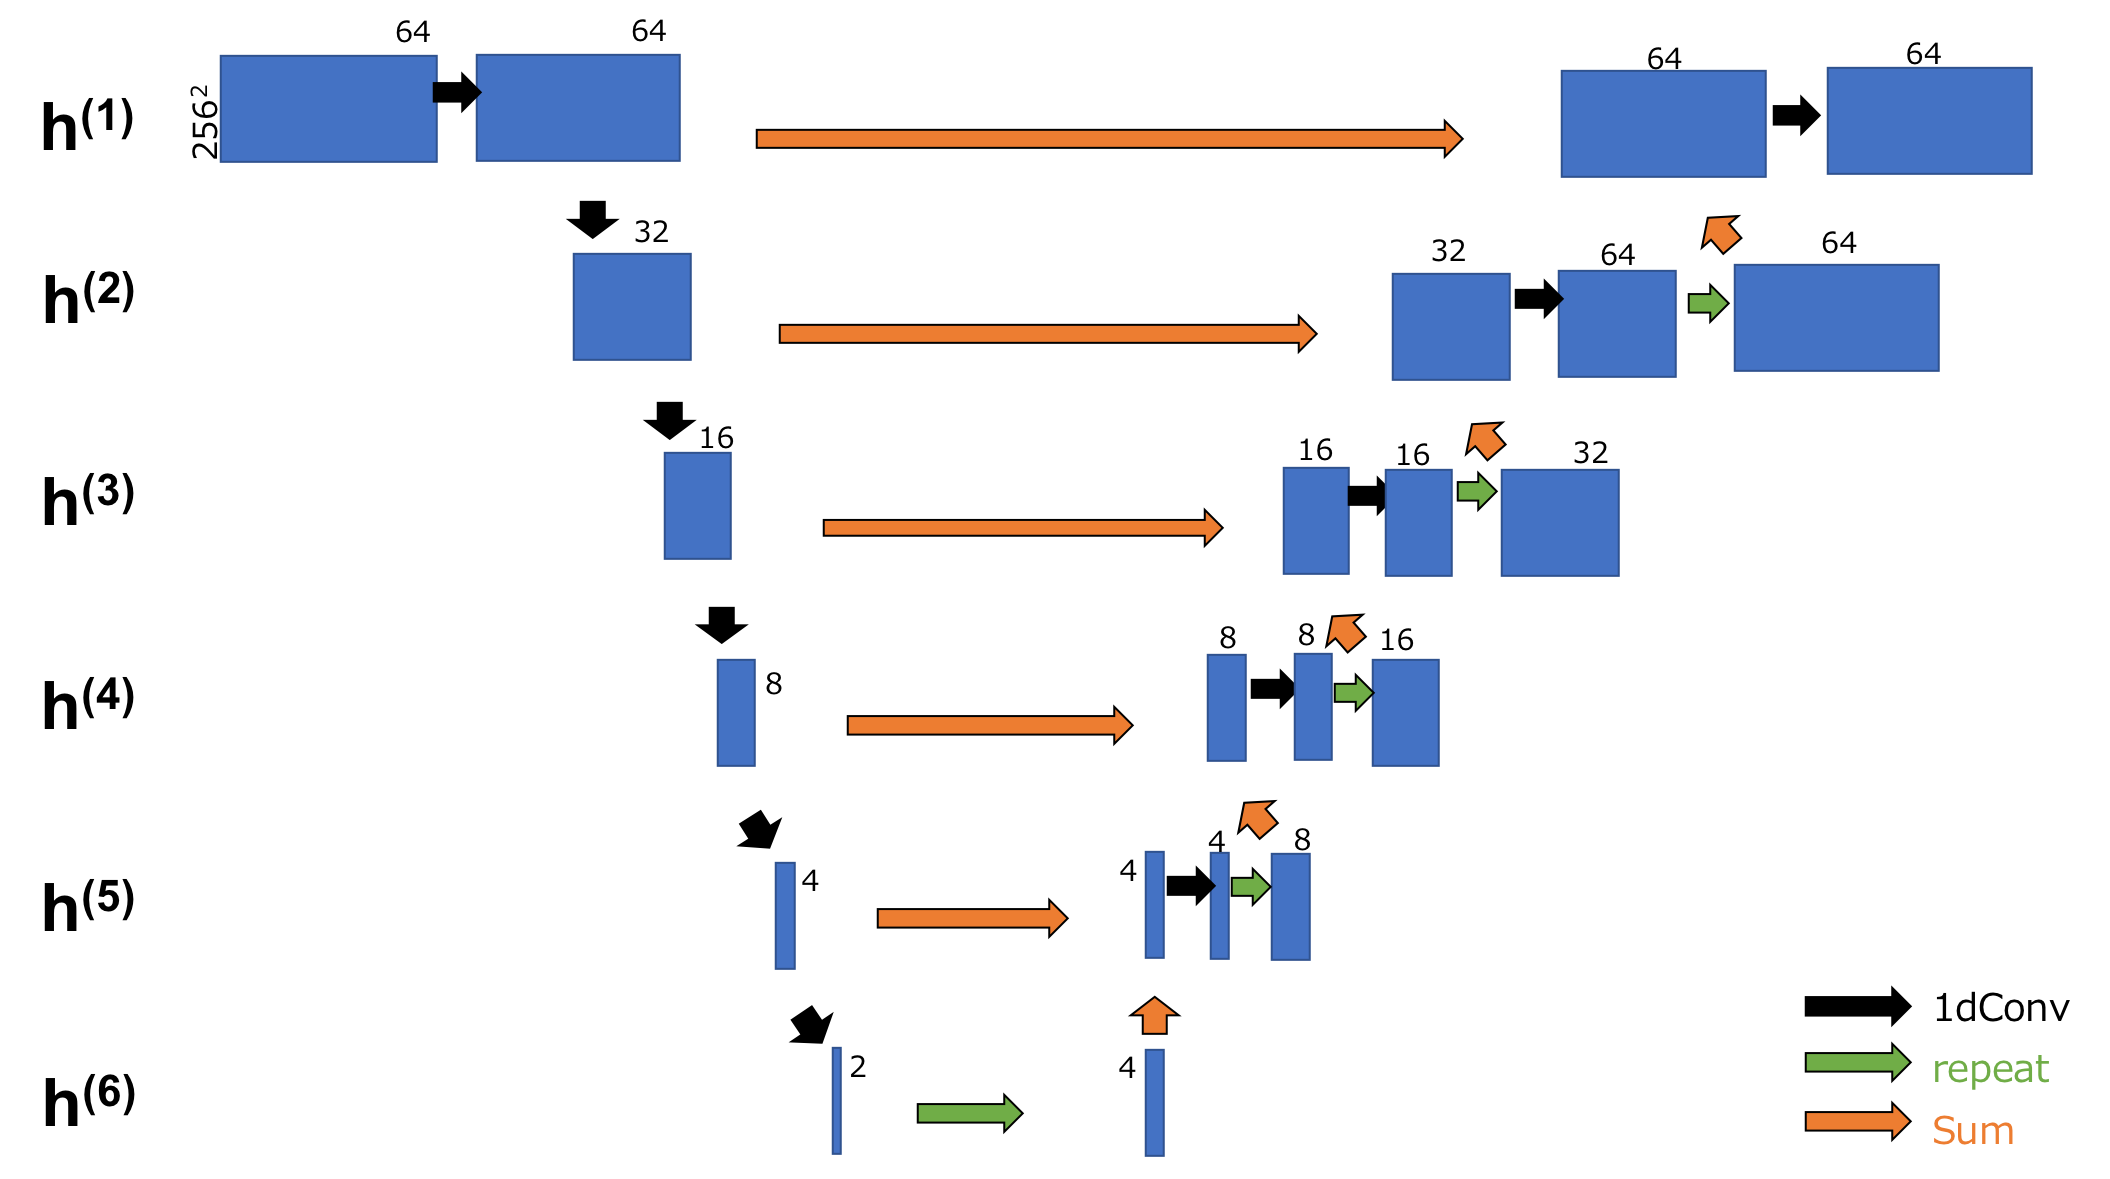
\includegraphics[width=6cm]{net_example.png}
  \caption{ネットワークの概要図}\label{tab:flowchart}
 \end{center}
\end{figure}

\vspace{-6mm}
\subsection{〇〇処理}
\vspace{-2mm}

〇〇処理

\vspace{-6mm}
\subsection{評価実験及び結果}
\vspace{-2mm}
本研究では,〇〇を定量的に評価する.

hogehogeは各出力データと正解データにおける頂点の座標の差の平均であり,式(\ref{eq:hoge})のように求められる.
\vspace{-6mm}

\begin{align}
hoge = \frac{1}{N\times64} \sum_{t=0}^N\sum_{i=0}^{64} (||\bar{x}_{t,i} -x_{t,i}||_2)
\label{eq:hoge}
\end{align}

\vspace{-2mm}

結果を表\ref{tb:example}に示す.
\begin{table}[h]
\caption{評価実験の結果} 
\label{tb:example}
\scalebox{1}[1]{
\hbox to\hsize{\hfil
\begin{tabular}{c|c|c}\hline
手法 & hoge1 & hoge2\\\hline\hline
従来手法\cite{hasegawa} & 8.618 & 0.432\\\hline
提案手法 & \textbf{8.263} & \textbf{0.511}\\\hline
\end{tabular}\hfil}}
\end{table}

結果として,hoge1,hoge2の両方において提案手法は最も良い結果を示した.

\vspace{-6mm}
\section{まとめ}
\vspace{-2mm}
まとめ

\vspace{-6mm}
\begin{scriptsize}
\addcontentsline{toc}{chapter}{\numberline{}参考文献}
\bibliographystyle{junsrt}
\begin{thebibliography}{10}
\bibitem{hasegawa} Minori Hasegawa:“title", In Proceedings of gakkaimei. 〇〇, pp. 79-86.

\end{thebibliography}
\vspace{3mm}
\vspace{-3mm}
%%%%%%%%%%%%%%%%%%%%%%%%%%%%%%%%%%%%%%%%%%%%%%%%%%%%%%%%%%%%%%%%%%%%%%%%%%% 
\begin{large}
\noindent {\bf 研究業績}
\end{large}
\addcontentsline{toc}{chapter}{\numberline{}研究業績}
\begin{description}
\item[(101)] name, 教授名:“title”, 平成〇〇処理年〇〇大会. 〇〇処理, pp. 220–221.
\item[(102)] name, 教授名:“title”, 平成〇〇処理年〇〇大会. 〇〇処理, pp. 220–221.
\item[(103)] name, 教授名:“title”, 平成〇〇処理年〇〇大会. 〇〇処理, pp. 220–221.
\end{description}
\end{scriptsize}
\end{document}
